% Intended LaTeX compiler: pdflatex
\documentclass[10pt,a4paper,UTF8]{article}
\usepackage{zclorg}
\author{张朝龙}
\date{}
\title{练习:向量空间的积与商}
\hypersetup{
 pdfauthor={张朝龙},
 pdftitle={练习:向量空间的积与商},
 pdfkeywords={},
 pdfsubject={},
 pdfcreator={Emacs 25.0.50.1 (Org mode 9.0.5)}, 
 pdflang={English}}
\begin{document}

\maketitle
\tableofcontents
\titlepic{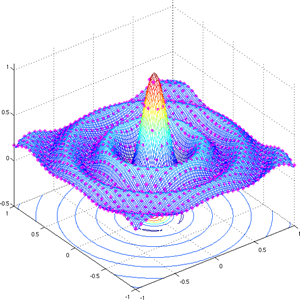
\includegraphics[scale=0.25]{../../img/sinc.PNG}}

\section{3.E.1}
\label{sec:org0d46596}


\begin{problem}
设\(T\)是\(V\)到\(W\)的函数。定义\(T\)的 \textbf{图} 为\(V\times W\)的如下子集:\[\{(v,Tv)\in V\times W:v\in V\}\]
证明\(T\)是线性映射当且仅当\(T\)的图是\(V\times W\)的子空间。
\end{problem}

\begin{answer}
正式的将,\(V\)到\(W\)的函数\(T\)是\(V\times W\)的一个子集\(T\),使得对于每个\(v\in V\)都有一个元素\((v,w)\in T\),也就是说,函数正式的讲就是上面所谓的图。我们通常并不把函数看成上面的这种正式形式。然而,如果采用上面的正式形式,则本题可以重述为:证明\(V\)到\(W\)的函数\(T\)是线性映射当且仅当\(T\)是\(V\times W\)的子空间。

假设\(T\)是线性映射则,对于\(u,v\in V, \lambda \in \mathbf{F}\)有:\(T(u+v) = Tu + Tv, T(\lambda u) = \lambda Tu\).

基对于\((u,Tu),(v,Tv)\in T\),则有\((u+v,T(u+v)) \in T\),齐次性的证明类似。

所以我们可以从\(T\)是线性映射推出\(T\)的图是\(V\times W\)的子空间。

另一方面,假设 T 的图是\(V\times W\)的一个子空间,则对于\((v,Tv),(u,Tu)\)有\((u+v,T(u+v))\)也属于\(T\)的图,根据线性映射的定义有\(Tv+ Tw = T(v+W)\)。另外\(T\)的齐次性证明类似。

综上,命题得证。
\end{answer}
\section{4.E.2}
\label{sec:orgdcf6fbd}



\begin{problem}
设\(V_{1},\ldots ,V_{m}\)均为向量空间使得\(V_{1}\times \ldots \times V_{m}\)是有限维的。证明对于每个\(j=1,\ldots ,m\)来讲\(V_{j}\)是有限维的。
\end{problem}

\begin{answer}
根据 3.76,命题得证。\(\dim (V_{1}\times V_{2} \ldots \times V_{m}) = \sum_{j=1}^{m}\dim V_{j}\)
\end{answer}

\section{3.E.7}
\label{sec:org8e42c7e}


\begin{problem}
设\(v,x\in V\),\(U,W\)是\(V\)的子空间,\(v+U = x + W\),证明\(U = W\)
\end{problem}

\begin{answer}
这种问题的证明一般是先证明\(U\subseteq W\),然后\(W\subseteq U\).

首先我们证明\(U\subseteq W\)。因为\(v+U = x + W\),则存在\(w_{1}\in W\)使得\(v = x+ w_{1}\)。所以有\(v-x \in W\),对于任何的\(u\in U\),存在\(w_{2}\in W\)有\[v+u = x+ w_{2}\] 所以有:\[u = (x-v) + w_{2}\in W\]
所以有\(U\subseteq W\)。类似的有\(W\subseteq U\)
\end{answer}

\section{3.E.8}
\label{sec:orgdd632e2}


\begin{problem}
证明:\(V\)的非空子集\(A\)是\(V\)的仿射子集当且仅当对于所有的\(v,w\in A\)和\(\lambda \in \mathbf{F}\)均有\(\lambda v + (1-\lambda)w \in A\)
\end{problem}

\begin{answer}
首先假设\(A\)是\(V\)的一个仿射子集,则存在\(a\in V\)和\(V\)的子空间\(U\),使得\(A = a+ U\)。对于\(A\)中的任何向量\(v,w\)都存在\(u_{1},u_{2}\in U\)可以写成\(v = a+ u_{1}\),\(w = a+ u_{2}\).因此:
\[\lambda v + (1-\lambda)w = a + [\lambda u_{1} + (1-\lambda)u_{2}] \in a + U = A\]

另一方面,因为\(A\)非空,假设\(a\in A\),只要我们证明\[A-a = \{x-a:x\in A\}\] 是\(V\)的一个子空间。因为只要证明\(A-a\)是\(V\)的子空间,则\(A = a+A-a\),我们就可以得到\(A\)是\(V\)的仿射子集。

对于\(x-a\in A -a\),\(\lambda \in \mathbf{F}\),那么:
\begin{equation}
\label{eq:1}
\lambda x + (1-\lambda)a \in A \rightarrow \lambda(x-a) = \lambda x + (1-\lambda)a -a \in A -a
\end{equation}

这意味着\(A-a\)标量乘法封闭。对于\(x-a\in A-a\)和\(y-a\in A-a\),其中\(x,y\in A\),我们有:
\(\frac{x}{2} + \frac{y}{2} -a \in A -a\) 因为\(A-a\)在标量乘法下封闭,所以\[(x-a) + (y-a) = 2(x/2 + y/2 -a) \in A-a\]

即,\(A-a\)加法封闭,所以\(A-a\)是\(V\)的一个子空间。
\end{answer}
\section{3.E.9}
\label{sec:org515ab8a}


\begin{problem}
设\(A_{1}\)和\(A_{2}\)均为\(V\)的仿射子集。证明\(A_{1}\cap A_{2}\)是\(V\)的仿射子集或者空集。
\end{problem}

\begin{answer}
假设\(A_{1}\cap A_{2}  = \varnothing\),那么对于\(x,y\in A_{1}\cap A_{2}\) 和\(\lambda \in \mathbf{F}\),根据上一题,我们有:
\begin{equation}
\label{eq:2}
\lambda x + (1-\lambda)y \in A_{1}
\end{equation}
\begin{equation}
\label{eq:3}
\lambda x + (1-\lambda)y \in A_{2}
\end{equation}
,所以\(\lambda x + (1-\lambda)y \in A_{1} \cap A_{2}\)

再次利用上一题的结论,\(A_{1}\cap A_{2}\)是\(V\)的一个仿射子集。
\end{answer}
\section{3.E.10}
\label{sec:orgcdd6fd9}


\begin{problem}
证明\(V\)的任意一族仿射子集的交是\(V\)的仿射子集或者空集。
\end{problem}

\begin{answer}
证明过程如上一题。
\end{answer}
\section{3.E.11}
\label{sec:orgaca6923}


\begin{problem}
设\(v_{1},\ldots ,v_{m}\in V\),令:
\begin{equation}
\label{eq:4}
A = \{\lambda_{1}v_{1} + \ldots + \lambda_{m} v_{m}:\lambda_{1},\ldots ,\lambda_{m} \in \mathbf{F}, \lambda_{1} + \ldots + \lambda_{m} = 1\}
\end{equation}

\begin{enumerate}
\item 证明\(A\)是\(V\)的仿射子集。
\item 证明\(V\)的每个包含\(v_{1},\ldots ,v_{m}\)的仿射子集均包含\(A\)。
\item 证明有某个\(v\in V\)以及\(V\)的某个子空间\(U\)使得\(A = v+U\)且\(\dim U \leq m-1\)
\end{enumerate}
\end{problem}

\begin{answer}
\begin{enumerate}
\item 设\(v = \lambda_{1}v_{1} + \ldots + \lambda_{m}v_{m} \in A\),\(w = \eta_{1}v_{1} + \ldots + \eta_{m}v_{m} \in A\),其中\(\lambda_{1} ,\ldots ,\lambda_{m}\in \mathbf{F}\), \(\lambda_{1} + \ldots + \lambda_{m} = 1\),\(\eta_{1} ,\ldots ,\eta_{m}\in \mathbf{F}\), \(\eta_{1} + \ldots + \eta_{m} = 1\),
\end{enumerate}

对任意的\(\lambda \in \mathbf{F}\),有:
\begin{equation}
\label{eq:5}
\lambda v + (1-\lambda)w = \sum_{i=1}^{m}(\lambda\lambda_{i} + (1-\lambda)\eta_{i})v_{i}
\end{equation}
注意到:
\begin{equation}
\label{eq:6}
\sum_{i=1}^{m}(\lambda\lambda_{i} + (1-\lambda)\eta_{i}) = \lambda \sum_{i=1}^{m}\lambda_{i} + (1-\lambda) \sum_{i=1}^{m}\eta_{i} = \lambda + (1-\lambda) = 1
\end{equation}

所以有:\(\lambda v + (1-\lambda)w \in A\),根据第 8 题,我们有:\(A\)是\(V\)的仿射子集。

\textbf{这个问题} 告诉我们证明一个子集是仿射子集不一定要按照定义来,也可以从第 8 题的思路出发。

\begin{enumerate}
\item 接下来使用数学归纳法来证明对人包含\(v_{1},\ldots ,v_{m}\)的仿射子集包含\(A\).
\end{enumerate}

对于\(k\leq m\),如果\(\sum_{i=1}^{k}\lambda_{i} = 1\),我们有:
\begin{equation}
\label{eq:7}
\sum_{j=1}^{k}\lambda_{j}v_{j} \in W
\end{equation}

对于\(k=1,2\),根据 3.E.8,我们有命题成立。

假设对于\(k\)命题成立,则对于\(k+1\leq m\),假设有\(\sum_{i}^{k+1}\lambda_{i} = 1\),如果\(\lambda_{k+1} = 1\),那么
\begin{equation}
\label{eq:8}
\sum_{j=1}^{k+1}\lambda_{j}v_{j} = v_{k+1} \in W
\end{equation}

如果\(\lambda_{k+1} \neq 1\),那么:
\begin{equation}
\label{eq:9}
\frac{1}{1-\lambda_{k+1}}(\lambda_{1}v_{1} + \ldots + \lambda_{k}v_{k}) \in W
\end{equation}

也就是说:
\begin{equation}
\label{eq:10}
\lambda_{1}v_{1} + \ldots + \lambda_{k+1}v_{k+1} \in W
\end{equation}

所以\(\lambda_{1}v_{1} + \ldots + \lambda_{m}v_{m}\in W\)

\begin{enumerate}
\item 因为\(\lambda_{1} + \ldots \lambda_{m} = 1\),那么:
\end{enumerate}
\begin{equation}
\label{eq:11}
\lambda_{1}v_{1} + \ldots + \lambda_{m}v_{m} = v_{1} + \lambda_{2}(v_{2} -v_{1}) + \ldots + \lambda_{m}(v_{m} - v_{1})
\end{equation}
因此\(A\subseteq v_{1} + span(v_{2} - v_{1},\ldots ,v_{m}-v_{1})\), \(v\)可以写为另外一种形式:
\begin{equation}
\label{eq:12}
v_{1} + \sum_{j=2}^{m}\lambda_{i}(v_{i} - v_{1}) = (1-\lambda_{2} - \ldots -\lambda_{m}) + \sum_{i=2}^{m}\lambda_{i}v_{i}
\end{equation}
注意:\(1-\lambda_{2} - \ldots -\lambda_{m} + \sum_{j=2}^{m}\lambda_{i} = 1\),所以
\begin{equation}
\label{eq:13}
v_{1} + span(v_{2}-v_{1},\ldots ,v_{m} - v_{1}) \subseteq A
\end{equation}

继而有:
\begin{equation}
\label{eq:14}
A = v_{1} + span(v_{2} - v_{1},\ldots ,v_{m}-v_{1})
\end{equation}
令\(v=v_{1}\),\(U = span(v_{2} -v_{1})\),则有\(\dim U \leq m-1\)
\end{answer}
\section{3.E.12}
\label{sec:org5a314c7}


\begin{problem}
设\(U\)是\(V\)的子空间使得\(V/U\)是有限维的。证明\(V\)同构于\(U\times (V/U)\)
\end{problem}

\begin{answer}

\end{answer}
\section{3.E.13}
\label{sec:org1eba348}


\begin{problem}
设\(U\)是\(V\)的子空间,\(v_{1} + U,\ldots ,v_{m} + U\)是\(V/U\)的基,\(u_{1},\ldots ,u_{n}\)是\(U\)的基,证明\(v_{1},\ldots ,v_{m},u_{1},\ldots ,u_{n}\)是\(V\)的基。
\end{problem}

\begin{answer}

\end{answer}
\end{document}
